\section{Experiments}
\label{sec:experiments}
Porting the models to the new framework is only the first part of the project. It is also important that these models, once ported, are able to perform in the exact same way as the original code would. The best way to verify that it does, is to repeat a set of experiments and compare the results to the original implementation. A couple of exemplary experiments were picked out for this purpose. Additionally, another simple test was also devised in order to benchmark the performance of this framework.

\subsection{Repeating ArtDev3D's experiments}
For this model, the sphere and the x-mas tree was chosen to test the new implementation. The reason for this is because the sphere is a relatively simple shape to evolve and easily achieve perfect fitness. For the second test, we will see how well the new implemention will do on difficult shapes.

Both of these experiments were conducted with different settings in order to see how parameters would affect the fitness of the individuals. In this thesis, however, I used a fixed set of parameters for simplicity's sake. The numbers may therefore deviate from the original results. Both of these experiments are run with settings as close to the original experiments as possible:

\begin{itemize}
	\itemsep=-2pt
	\item Population: 1 000
	\item Generations: 500
	\item Mating rate: 90\%
	\item Mutation rate: 10\%
	\item Crossover: Single point
	\item Selection: Tournament (size=4, pressure=0.8)
\end{itemize}

And the parameters used for development:

\begin{itemize}
	\itemsep=-2pt
	\item Development time: 12 ticks
	\item Protein lifespan: 5 ticks
	\item Cell types: 1 (sphere) / 12 (x-mas tree)
	\item Chemical types: 1
	\item Don't-care-neighbours: 6
\end{itemize}

\subsubsection{Sphere}
This shape seems the simplest to evolve as it is entirely symmetrical and much less complex than other shapes. Since these experiments are about verifying that everything runs as it should, they will always use the same parameters. 200 runs were conducted, and the number of perfect specimens found was recorded.

\begin{center}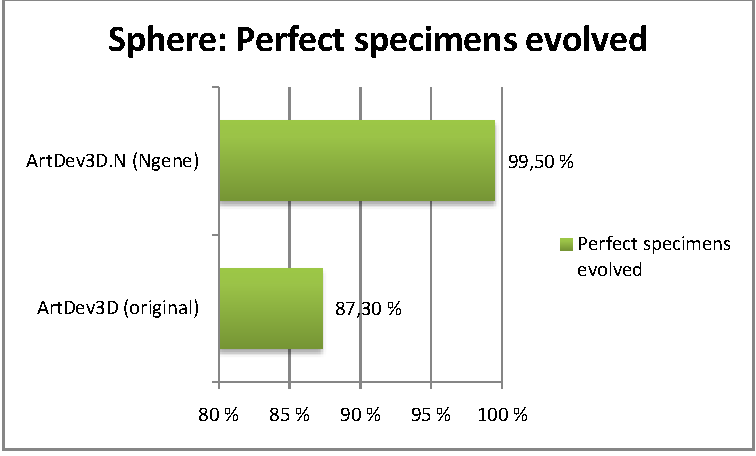
\includegraphics[scale=0.9]{chart_artdev3d_sphere}\end{center}

Original ArtDev3D managed to evolve perfect fitness 856 out of 980 experiments. It is important to remember that these were run with \emph{different} settings whereas we are using the best settings available here. That is why we see a much higher percentage (199 out of 200) than the original experiments. Had we known what these parameters were beforehand and used them, the number would probably have been much closer to the original results. Regardless, it does show that Ngene can perform equally well.

\subsubsection{X-mas tree}
This experiment is of a different nature than the previous one. It may not be very scientific but should demonstrate how well Ngene performs on complex shapes compared to ArtDev3D. No perfect specimens are expected here because ArtDev3D had a hard time evolving one, and it is not expected for Ngene to outperform it. As with previous test, 200 runs were conducted. The highest fitness after each run was recorded for the following graph.

\begin{center}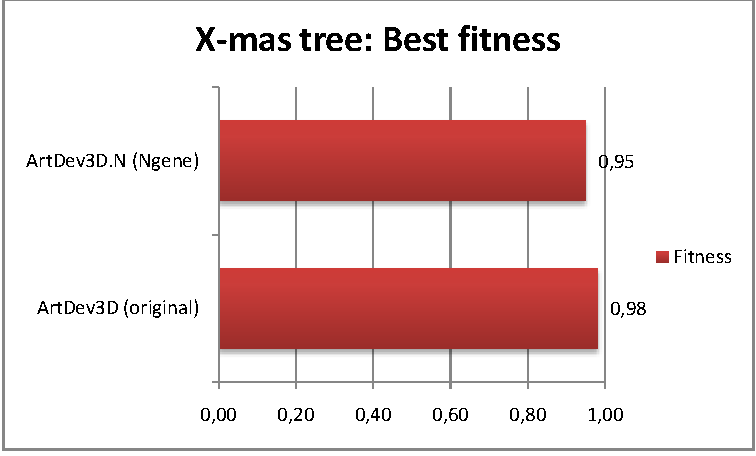
\includegraphics[scale=0.9]{chart_artdev3d_x-mas-tree}\end{center}

It seems that Ngene is performing rather well. Note that the highest fitness achieved in ArtDev3D only occured once in the 980 test runs conducted. This experiment is but a fifth of that, and it is not inconceivable that Ngene might be able to achieve higher fitness with a larger sample. Interestingly, Ngene only managed to evolve fitness above 0.9 in 57 out of 200 runs. The rest were above 0.8 however.

\subsubsection{Summary}
We've seen that Ngene's implementation of ArtDev3D can evolve on an equal level as the original implementation. In chapter~\ref{sec:Implementation:ArtDev3D}, I've mentioned that there was a fix applied to the engine when it was ported to the framework. From what can be seen above, it would seem that this patch has not affected the model in any perceivable way. Whether or not the fix is beneficial in any way, is difficult to see. It may very well be that the bug is dormant.


\subsection{Repeating a cartesian genetic programming experiment}
For the CGP model, the French flag experiment was picked out. The purpose of this experiment is to evolve a grid of cells that resembles the French flag. Each cell is given a type of either blue, red or white. For every cell that corresponded with the target, one point was rewarded. The fitness is calculated from the total points scored divided by maximum score achievable. The engine ran with the following settings:

\begin{itemize}
	\itemsep=-2pt
	\item Population: 100
	\item Generations: 10 000
	\item Mating rate: 90\%
	\item Mutation rate: 30\%
	\item Crossover: Single point
	\item Selection: Tournament (size=4, pressure=0.8)
\end{itemize}

The target phenotype used:

\begin{center}\fbox{
\includegraphics[scale=0.9]{French-flag}}\end{center}

Finding the right development time for this particular problem proved to be rather difficult. It would seem that setting the development time too high not only slowed down the whole process, it also made it harder for the organisms to evolve correctly. The experiments started out with development time of 10 ticks and was slowly decremented as the results were not satisfactory. The following are the best evolved organisms using 4 ticks.

\begin{center}
	\fbox{
\includegraphics[scale=0.9]{cartesian-4-3-90-9-3-20081119-083309}}
	~\fbox{
\includegraphics[scale=0.9]{cartesian-4-3-90-9-3-20081119-091139}}
	~\fbox{
\includegraphics[scale=0.9]{cartesian-4-3-90-9-3-20081119-230852}}
\end{center}

It seemed odd that setting the development time one step longer would have any saying in how the organisms would grow. To ensure that the results weren't purely coincidential, the experiment was repeated once more for five ticks.

\begin{center}
	\fbox{
\includegraphics[scale=0.9]{cartesian-5-3-90-9-3-20081120-221123}}
	~\fbox{
\includegraphics[scale=0.9]{cartesian-5-3-90-9-3-20081120-233001}}
	~\fbox{
\includegraphics[scale=0.9]{cartesian-5-3-90-9-3-20081121-002613}}
\end{center}

These results seem to suggest that the model is not stable. Colours appear in areas they shouldn't be in as opposed to the previous results where the colours at least stayed closer to each other. One can theorize that the growth continues even after target phenotype have been evolved, hence resulting in a worse fitness. This seems to be backed up by the fact that the engine would more frequently obtain fitness above 0.9 when using development time of four when compared to five. Using development time of 10 also raised the number of cells above 200.

To further investigate this issue, the phenotype was altered so that it would have a border around the flag.

\begin{center}\fbox{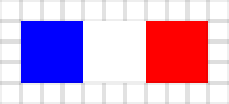
\includegraphics[scale=0.9]{French-flag-border}}\end{center}

This new phenotype will hopefully show whether or not the model does continue to grow, or if it manages to maintain a status quo to some extent. No changes were made to the settings above. The tests were repeated using the new target phenotype.

\begin{center}
	Development time: 4 ticks\newline
	\fbox{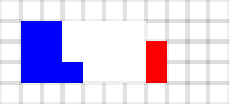
\includegraphics[scale=0.9]{cartesian-4-3-90-9-3-20081120-071044}}
	~\fbox{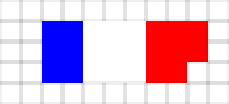
\includegraphics[scale=0.9]{cartesian-4-3-90-9-3-20081120-081439}}
\end{center}

\begin{center}
	Development time: 5 ticks\newline
	\fbox{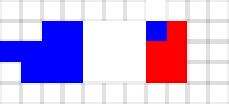
\includegraphics[scale=0.9]{cartesian-5-3-90-9-3-20081121-063215}}
	~\fbox{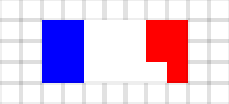
\includegraphics[scale=0.9]{cartesian-5-3-90-9-3-20081121-072947}}
	~\fbox{
\includegraphics[scale=0.9]{cartesian-5-3-90-9-3-20081121-205507}}
\end{center}

As suspected, the average fitness dropped due to the increased size and complexity of the phenotype. With the exception of the first flag in the second row that ``bleeds'' into the border (two cells: blue on the left and white cell above the one blue cell in red cells zone), all of them are missing cells for some reason. It seems like the model compensates by either growing less cells or initiating cell death more often. Unfortunately, the results can't be called conclusive due to the nature of test. One will have to look into how the organisms change in each development step. The tools necessary for this is unavailable at the moment.

Another interesting thing to note is that the bug mentioned in section~\ref{sec:cartesian} had little to no effect on any of the results above. In fact, the no-bug version seem to achieve higher fitness more frequently than the bugged version by a small margin. This conflicts with what Dr. Miller reported.


\subsection{Performance benchmarks}
With regards to what has been written about ArtDev3D up to this point, I've only discussed the potential performance gain of this framework without showing anything concrete. We shall now put these claims under scrutiny, and see how fast the new ArtDev3D, cleverly dubbed ArtDev3D\emph{.N} (N for Ngene or N-hanced), really is. This simple benchmark test was run on an Intel\textregistered Core\texttrademark 2 Duo E6300 with 2 GB of DDR2-RAM under Linux 2.6.27-7. The conditions of the programs under run:

\begin{itemize}
	\itemsep=0pt
	\item ArtDev3D ran with Java\texttrademark SE Runtime Environment 6 Update 10 build 33.
	\item ArtDev3D.N was compiled with GCC 4.3.2, with optimization flags: \texttt{-O3}.
	\item Additionally, ArtDev3D.N was also compiled with Intel\textregistered C++ Compiler (ICC) 11.0 build 069, with optimization flags: \texttt{-xHost -fast}.
\end{itemize}

The same settings were used for both engines:

\begin{itemize}
	\itemsep=-2pt
	\item Population: 100
	\item Generations: 100
	\item Mating rate: 90\%
	\item Mutation rate: 30\%
	\item Development time: 12 ticks
	\item Target: Sphere
\end{itemize}

Perfect termination was disabled so that the engines would not exit when perfect fitness was found. This is to ensure that both engines ran for the exact same number of generations. The test was repeated 100 times and the average time was then calculated.

\begin{center}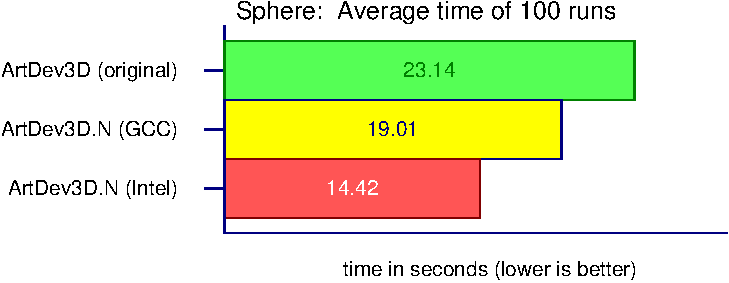
\includegraphics[scale=0.9]{chart_avg-time}\end{center}

The speed gained here is quite significant considering that the sample is relatively small to perform a benchmark on. Using an open source compiler such as GCC, Ngene is faster than ArtDev3D by 4.13 seconds. This is to be expected as C++ is faster than Java. We also see that switching to a better compiler like ICC shaved off an additional 4.59 seconds, making the gap 8.72 seconds. The optimizations flags were not experimented with so the gap could potentially be increased even more. The framework itself can still be optimized further as well. We will have the discussion regarding this topic in chapter~\ref{sec:improvements}. Speed aside, it is also interesting to see how they perform memory-wise. These numbers were taken during the experiments above.

\begin{center}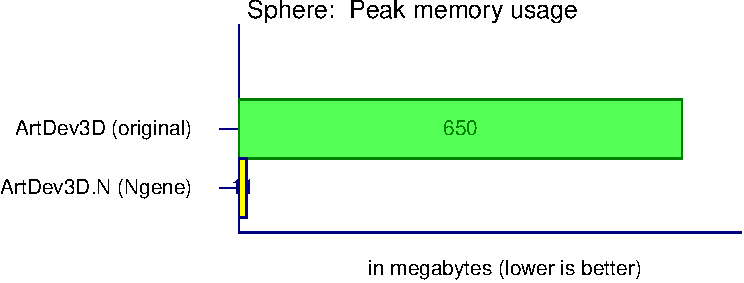
\includegraphics[scale=0.9]{chart_peak-memory-usage}\end{center}

ArtDev3D peaks at a staggering 650 MB! The average is only a few MB less. The main culprit for this is Java\texttrademark Virtual Machine. It has been criticized\cite{maio2008} for the garbage collector because of its ridiculous memory consumption. The reason behind is that during allocation and deallocation, it leaves the memory very fragmented and has a hard time filling the gaps in between, resulting in more memory allocated without being used entirely. Memory usage is important because lowering memory use can also increase overall performance. The computer that these experiments were conducted on has 2 MB of L2 cache. If a program fit into this cache, it would run significantly faster than a program that doesn't. Ngene peaks out at 11 MB but averages at around 7 MB during a run.
